\chapter{Observations}
\label{chap:observations}

 
% \begin{figure}[b]
%   \centering
%   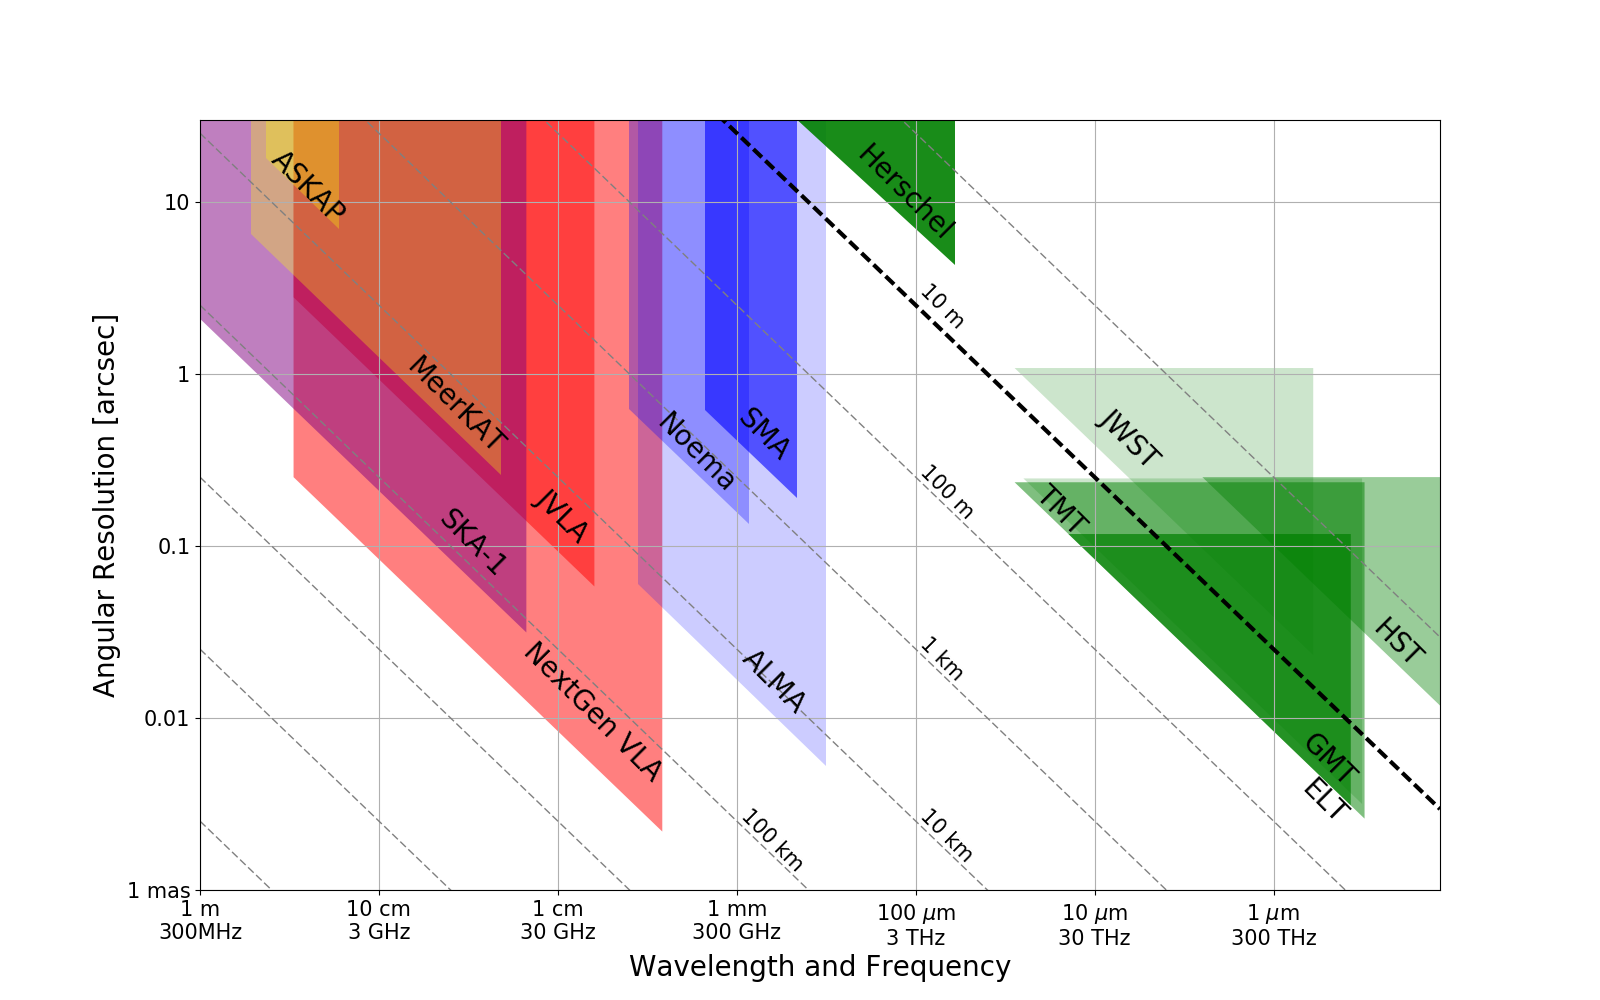
\includegraphics[width=\linewidth]{interferometers.png}
%   \captionof{figure}{Current and future radio interferometers, contextualized by their blah}
%   \label{fig:interferometers}
% \end{figure}


% What are these dishes of which you speak?  What are baselines and how do they tell you about angular scales?  What is a spectral window?  REWORK
The data presented in this thesis are part of an ALMA survey of Orion proplyds in Orion (project 2011.0.00028.S); data collection and analysis methods of the continuum results are presented in \citet{Mann2014}. The observations were taken on October 24, 2012, in ALMA's Band 7 receivers. Four spectral windows of width 1.875 GHz were arranged to cover the rest frequencies of the HCO$^+$(4-3), HCN(4-3), CO(3-2), and CS(7-6) transitions (356.734 GHz, 354.505 GHz, 345.796 GHz, and 342.883 GHz, respectively). Each window was split into 3840 channels with a width of 488.28 kHz, yielding a velocity resolution of 0.42 km s$^{-1}$. Since this was part of a Cycle 0 Early Science project, the survey used only 22 of the ALMA's 50 12 meter dishes in a hybrid configuration, with baselines ranging from 21.2 to 384.2 meters. This configuration yields a maximum angular scale of 8", angular resolution of 0."5, and beam FWHM of 15". At a Gaia-measured distance of 389 $\pm$ 7.97 \citep{GaiaCollaboration2018,GaiaCollaboration2018}\footnote{This measurement is nearer than the previous literature value of 414 pc.}, max angular scales and angular resolution correspond to 3,112 AU and 194 AU, respectively. The observation's pointing center was (05:35:25.30, -05:15:35.50). Each disk's precise position was fit for (see \S\ref{chap:analysis}), and are given in Table \ref{table:disk_positions}.


% REWORK: Make sure these numbers are right!
\begin{table}
  \centering
  \caption{Disk Positions}
  \label{table:disk_positions}
  \renewcommand{\arraystretch}{1.2}
  \begin{tabular}{c | c | c }
    \toprule \toprule
      Source      &  RA            & Dec \\
    \midrule %\midrule
      d253-1536a  &  $05:35:25.3002$ & $-05:15:34.418$  \\
      d253-1536b  &  $05:35:24.2940$ & $-05:15:35.800$  \\
    \bottomrule
  \end{tabular}
\end{table}

% From listobs:
% 05:35:25.30 & -05:15:35.50
% Offsets: [0.0002, 0.082], [-1.006, -0.3]
% sig figs on the distance
% For Gaia references: https://gea.esac.esa.int/archive/documentation/GDR2/bib.html#bib173




These data, from Field 4 of \citet{Mann2014} represent 13.6 minutes of on-source time. This duration was split into six 136 second observations, spaced out over 7.5 hours to ensure adequate \textit{uv} coverage, yielding an RMS of 7mJy/beam in the line data. The resulting synthesized beam has dimensions of of 0.57$\times$0.51 arcsec with a position angle of 85\degree. Precipitable water vapor in the atmosphere was stable at 0.7 mm, indicating that atmospheric contributions to the data were negligible.


% This section also needs more explanation.  What is a gain calibration?  A bandpass calibration?  Why quasars?  Same for flux calibration.  Why a solar system object?  These answers don’t have to be long, but you’ll need a few sentences to help out our non-radio-astronomer colleagues.  REWORK
The data were calibrated by ALMA staff using standard procedures in the Common Astronomy Software Applications, or CASA \citep{McMullin2007}. The antenna-based complex gains and bandpass response of the system were calibrated using observations of the quasars J0607-085 and J0522-364 respectively. The absolute flux calibration was determined from observations of Callisto. The model of Callisto was drawn from \citet{Butler2012}. Absolute flux calibration is estimated to be accurate to within ∼ 10\% \citep{Mann2014}.



The velocity reference frame was converted from CASA's standard topocentric frame to LSRK (kinematic local standard of rest) using the CASA task \texttt{cvel}. Next, continuum emission was subtracted from the data in the uv plane using the CASA task \texttt{contsub}. Visibilities were imaged with standard inversion, deconvolution, and restoration procedures from the Multichannel Image Reconstruction Image Analysis and Display, or MIRIAD, package \citep{Sault1995}.





% Note that no closing info is needed.
